\documentclass{standalone}
\usepackage{tikz}
\usepackage{pgfplots}
\pgfplotsset{compat=newest}
\usepackage{pgfmath}
\usepackage{tikz-cd}
\usepackage{pgffor}
\usepackage{tkz-euclide}
\usetkzobj{all}
\usepgfplotslibrary{fillbetween}
\usetikzlibrary{
	calc,
	angles,
	quotes,
	arrows.meta,
	decorations.markings,
	math,
	backgrounds,
	pgfplots.statistics,
	matrix,
	patterns,
	shapes.geometric,
	spy,
	intersections,
}
\begin{document}
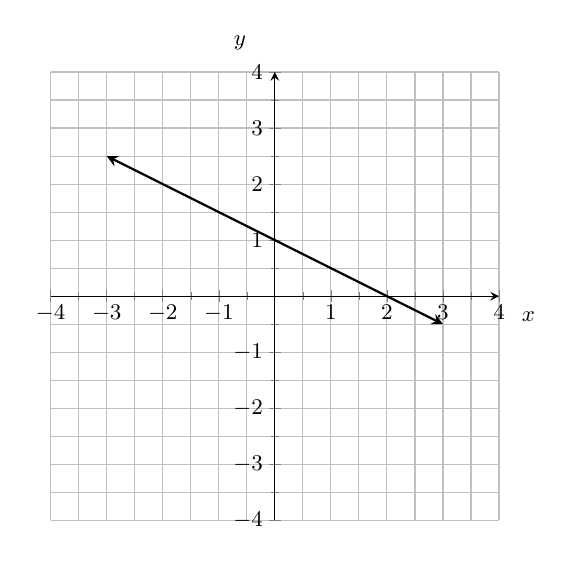
\begin{tikzpicture}[scale=1, every node/.style={scale=0.9}]
\begin{axis}[
grid=both,
unit vector ratio=1 1 1,
ymin=-4,
ymax=4,
xmax=4,
xmin=-4,
xtick={-10,-9,...,9,10},
ytick={-10,-9,...,9,10},
minor tick num=1,
axis lines = middle,
xlabel=$x$,
ylabel=$y$,
x tick label style={yshift=0.5ex,font={\small}},
y tick label style={xshift=0.25ex, font={\small}},
label style ={at={(ticklabel cs:1.1)},
font={\small}}
]
\addplot[thick, samples=100,domain=-3:3, name path=A, stealth-stealth]   {-1/2*x+1};
\end{axis}
\end{tikzpicture}
\end{document}